% !TeX spellcheck = en_US
\documentclass[letterpaper,12pt,twoside]{report}
\usepackage{fancyhdr}
\usepackage{fullpage}
\usepackage{tikz}
\usepackage{amsmath}

\begin{document}
	\pagestyle{fancy}
	\fancyhf{}
	\fancyhead[L]{Day 24}
	\fancyhead[R]{\textit{The Calendar Project}}
	\fancyfoot[L]{Citations Involved: none}
	
	% Problem
	\paragraph{Problem}
	\begin{quote}
		\textsf{In square $ABCD$, $M$ is the
			midpoint of $\overline{DC}$. If a side of $ABCD$ has
			length of 10cm, what is the area of the
			circle that passes through $A$, $B$, and $M$?}
	\end{quote}
	
	% Graphics
	\begin{center}
		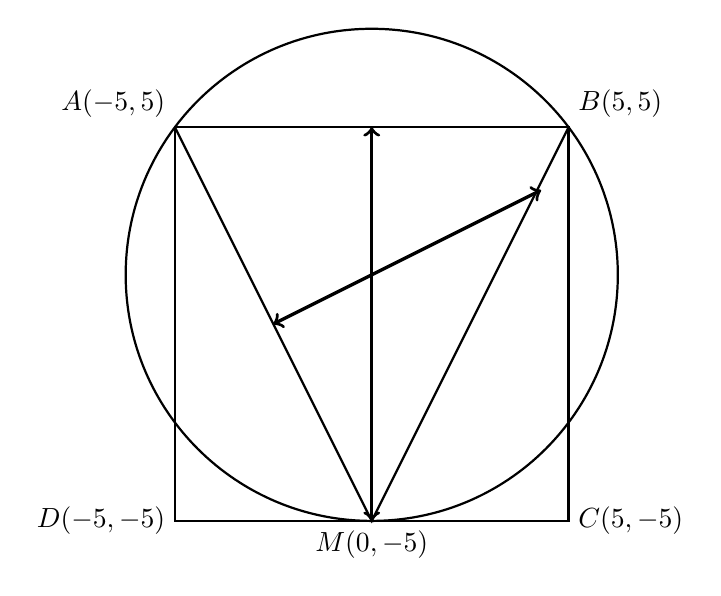
\begin{tikzpicture}[scale=0.5]
		
		\draw[thick] (-5,5) -- (5,5) -- (5,-5) -- (-5,-5) -- cycle;
		\node[above left] at (-5,5) {$A(-5,5)$};
		\node[above right] at (5,5) {$B(5,5)$};
		\node[right] at (5,-5) {$C(5,-5)$};
		\node[left] at (-5,-5) {$D(-5,-5)$};
		
		\draw[very thick, <->] (0,5) -- (0,-5);
		\draw[very thick, <->] (-2.5,0) -- (4.3,3.4);
		
		\draw[thick] (-5,5) -- (0,-5) -- (5,5);
		\node[below] at (0,-5) {$M(0,-5)$};
		\draw[thick] (0,1.25) circle [radius=6.25];
		
		\end{tikzpicture}
	\end{center}
	
	% Reasoning
	\paragraph{Reasoning}
	\begin{quotation}
		
		By the definition of triangle circumscription, the circle that contains $A$, $B$, and $M$ circumscribes $\triangle ABM$. The center of the circumscribed circle is the circumcenter, which can be determined by solving for the point of intersection of the perpendicular bisectors of two of the triangle's sides.
		
		Position the figure described in the 2D Euclidean coordinate plane such that the coordinate of each vertex matches the denoted values above. Given that $M$ is the midpoint of $\overline{DC}$, its coordinates are $(\frac{-5+5}{2},\frac{-5+(-5)}{2})=(\frac{0}{2},\frac{-10}{2})=(0,-5)$ by the Midpoint Formula.
				
		The midpoint of $\overline{AB}$ is $(\frac{x_1+x_2}{2},\frac{y_1+y_2}{2})=(\frac{-5+5}{2},\frac{5+5}{2})=(0,5)$ according to the Midpoint Formula. The slope of $\overline{AB}$ is $\frac{y_2-y_1}{x_2-x_1}=\frac{5-5}{5-(-5)}=\frac{0}{10}=0$ according to the Slope Formula. The opposite reciprocal of 0, the slope of the perpendicular bisector of $\overline{AB}$, is undefined. A line with undefined slope that passes through $(0,5)$ has an equation of $x=0$ [!].
		
		The midpoint of $\overline{MB}$ is $(\frac{x_1+x_2}{2},\frac{y_1+y_2}{2})=(\frac{0+5}{2},\frac{5+(-5)}{2})=(\frac{5}{2},\frac{0}{2})=(2.5,0)$. The slope of $\overline{MB}$ is $\frac{y_2-y_1}{x_2-x_1}=\frac{5-(-5)}{5-0}=\frac{10}{5}=2$. The opposite reciprocal of 2 is $-\frac{1}{2}$, which is the slope of the perpendicular bisector of $\overline{MB}$. The equation for this perpendicular bisector is $y-0=-\frac{1}{2}(x-2.5)$ in point-slope form.
		
		To solve for the point of intersection of the perpendicular bisectors, their equations are combined in a system of equations: $x=0$ and $y=-\frac{1}{2}(x-2.5)$. After substitution, $y=-\frac{1}{2}(0-2.5)=-\frac{1}{2}(-2.5)=\frac{2.5}{2}=1.25$. The point of intersection is therefore at $(0,1.25)$. This is the circumcenter of $\triangle ABM$, meaning that it is the center of the circumscribed circle, whose radius is the distance from its center to one of the triangle's vertices. Since $M$ also lies on the Y axis, it is the most convenient vertex for use in determining the radius of the circle, which is deduced using the Distance Formula: $\sqrt{(x_2-x_1)^2+(y_2-y_1)^2}=\sqrt{(0-0)^2+(-5-1.25)^2}=\sqrt{39.0625}=6.25$.
		
		The area formula for a circle is $r^2 \pi$ where $r$ is its radius. With the circumscribed circle's radius equal to 6.25, its area is $r^2\pi=6.25^2\pi=\boxed{39.0625\pi\approx 122.718463 \text{  cm}^2}$.
		
	\end{quotation}
	
	\paragraph{External References}
	
	\begin{enumerate}
		\item Textbook Ch. 3, Pg. 184: Opposite Reciprocals
		\item Textbook Ch. 5, Pg. 308: Definition of Triangle Circumscription / Finding the Circumcenter of a Triangle
		
		
	\end{enumerate}
	
\end{document}